\documentclass[]{article}
\usepackage{textcomp}
\usepackage{amssymb}
\usepackage{datetime}
\usepackage{graphicx}
\usepackage{geometry}
\usepackage{caption}
\usepackage{multicol}

\geometry{textwidth = 17cm,textheight = 24cm}

\begin{document}

%-------------------- begin header -------------------%
\centerline{\LARGE Process sheet for \textbf{stf\_res\_01}}
\vspace{0.5em}
\centerline{\Large Physics and Hardware for Intelligence project}
\vspace{0.5em}
\centerline{\large Physical Measurement Laboratory, NIST Boulder}
\vspace{0.5em}
\centerline{Dated \today}
%-------------------- end header ---------------------%

\begin{figure}[!h]
\centering
\setlength{\fboxsep}{0pt}%
\setlength{\fboxrule}{0pt}%
\fbox{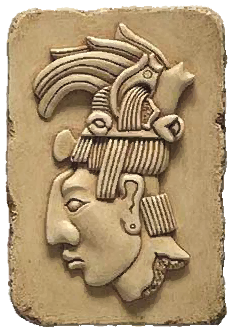
\includegraphics[width=3cm]{figures/votan_white.png}}
%\caption*{Votan, the Mayan god of optical to electrical transduction.}
\end{figure}

\begin{abstract}
Fabrication flow for the SPD/JJ integration process. WSi SNSPDs are integrated with Nb/Si/Nb, externally shunted JJs. This process includes the superconducting thin-film layer and associated Nb wiring and Au resistors, a ground plane, the JJ tri-layer stack and associated PdAu shunt resistor layer, and an upper Nb wiring layer.

The process starts with a thermally oxidized Si wafer with 160\,nm SiO$_2$. 

The entire wafer is clad with oxide, and openings are etched to the bond pads (\textbf{v4}). A Nb ground plane is deposited, and alignment marks are etched in this layer. Features are then etched in the ground plane (\textbf{m0}).

\vspace{2em}\noindent Insert screen shot of die and image distribution from stepper:
\vspace{1em}
\end{abstract}

\begin{multicols}{2}
\setcounter{tocdepth}{2}
\setcounter{secnumdepth}{4}
\tableofcontents
\end{multicols}
\newpage

\section{\label{sec:m1_dep}Deposit M1 (lower Nb wiring)}
\begin{itemize}
\item Begin with oxidized Si substrate
\item Deposit 120\,nm Nb with the Lesker SNS tool
\item Instructions for tool use: OneNote/a4/fab/SNS
\item Recipe: Nb\_wire\_js.rcp
\item Rate: 80\,nm/min; check log book for latest rate
\item Insert picture of log book entry
\end{itemize}

\newpage
\section{\label{sec:pm}PM (alignment marks)}
\begin{itemize}
\item Spin: SPR600 @ 3000\,rpm
\item Expose: 220\,mJ/cm$^2$
\item Develop: double puddle, 30\,s, 30\,s
\item Run through spin rinse dry
\item Inspect with microscope
\item Etch with Oxford fluorine ICP RIE
\begin{itemize}
\item Recipe: Nb PM He
\begin{itemize}
\item SF$_6$: 30\,sccm
\item RF: 25\,W
\item ICP: 800\,W
\item Pressure: 15\,mTorr
\item He: 5\,Torr
\end{itemize}
\item Etch: 70\,s
\item Typical DC bias: 60\,V @ 25\,W RF
\item No endpoint monitoring
\end{itemize}
\item Ash: 2\,min
\end{itemize}

\newpage
\section{\label{sec:m1}Pattern and Liftoff M1 (lower Nb wiring)}
\begin{itemize}
\item Begin with oxidized Si substrate
\item Pattern for liftoff:
\begin{itemize}
\item Ash: 2\,mins
\item Spin: LOR3A @ 4000\,rpm
\item Bake: 500\textcelsius\,\,for 5\,min
\item Spin: SPR600 @ 3000\,rpm, no P20
\item Expose: 220\,mJ/cm$^2$
\item Develop: double puddle, 30\,s, 30\,s
\item Run through spin rinse dry
\item Inspect with microscope
\end{itemize}
\item Deposit 60\,nm Nb with the Lesker SNS tool
\begin{itemize}
\item Instructions for tool use: OneNote/a4/fab/SNS
\item Recipe:  WR\_lf\_js.rcf in directory SNS-3gnI
\item Rate: 0.69\,nm/s; check log book for latest rate
\item Stress: -14.67\,MPa, compressive for 225\,nm film thickness (last measured 20200220
\item Insert picture of log book entry
\end{itemize}
\begin{itemize}




\item Recipe: 150mm\_Nb\_sloped\_ManEP
\begin{itemize}
\item SF$_6$: 40\,sccm
\item O$_2$: 16\,sccm
\item RF: cut after strikie
\item ICP: 500\,W
\item Pressure: 6.5\,mTorr
\item He: 4\,Torr
\item Rate: $\sim$\,0.51\,nm/s; $\sim$\,31\,nm/min
\item Note: Selectivity over resist is poor; limit to 300\,nm Nb to be etched
\end{itemize}
\item Etch: $\sim$230\,s
\item No DC bias
\item Use endpoint; typical signal shown in Fig.\,\ref{fig:plasmatherm_Nb_sloped_endpoint}
\item Insert picture of endpoint signal and log book entry
\end{itemize}
\item Ash: 2\,min
\item Clean: acetone dirty 2\,min, acetone clean 2\,min, IPA, spin rinse dry
\item Inspect with microscope
\item Measure thickness with profilometer
\end{itemize}





\newpage
\section{\label{sec:stf}STF (superconducting thin film)}
\begin{figure}[!h]
\centering
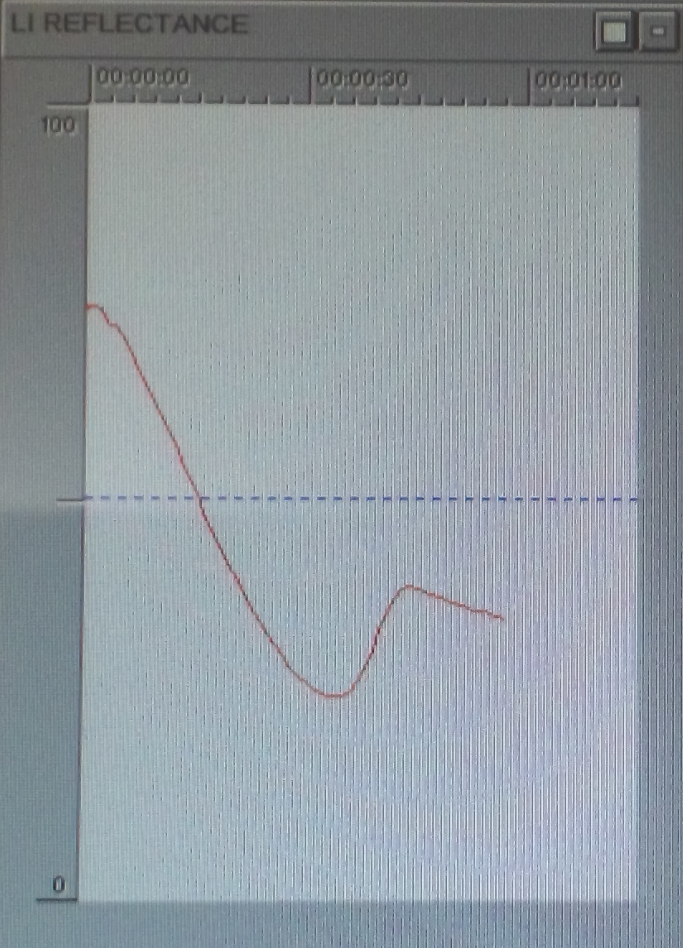
\includegraphics[width=14cm]{figures/oxford_MoSi_etch.png}
\caption{\label{fig:oxford_MoSi_etch}Typical endpoint signal of MoSi etch. The small peak after the dip is interpreted as the end of the etch. Overetch by 10\,s-20\,s after that peak.}
\end{figure}

\begin{itemize}
\item Ash 5\,min
\item Deposit MoSi in AJA
\item Recipe: MoSi \_ jms
\begin{itemize}
\item RF plasma clean for 150\,s at 80\,W
\item Typical DC voltage: 100\,V
\item Deposit MoSi: 50\,s
\item Voltage: 460\,V
\item Current: 440\,mA
\item Deposit a-Si: 66\,s
\item Voltage: 183\,V
\end{itemize}
\item Pattern
\begin{itemize}
\item Spin: SPR600 @ 3000\,rpm
\item Expose: 220\,mJ/cm$^2$
\item Develop: double puddle, 30\,s, 30\,s
\item Run through spin rinse dry
\item Inspect with microscope
\item Etch with Oxford Fl
\begin{itemize}
\item Recipe: opto-WSi-v2-lowHeForCarrier
\begin{itemize}
\item SF$_6$: 1\,sccm
\item Ar: 80\,sccm
\item RF: strike at 30\,W, cut to 10\,W as quickly as possible
\item ICP: 600\,W
\item Pressure: 10\,mTorr
\item He: 5\,Torr
\item Rate: $\sim$\,8\,nm/min
%\item Note: 
\end{itemize}
\item Etch: $\sim$60\,s-70\,s
\item DC bias: 67\,V
\item Use endpoint; typical signal shown in Fig.\,\ref{fig:oxford_MoSi_etch}
\item Insert picture of endpoint signal and log book entry
\end{itemize}
\item Ash: 2\,min
\item Clean: acetone dirty 2\,min, acetone clean 2\,min, IPA, spin rinse dry
\item Inspect with microscope
\end{itemize}
\end{itemize}

\newpage
\section{\label{sec:r1}R1 (Au resistors)}
\begin{itemize}
\item Pattern for liftoff
\begin{itemize}
\item Ash: 3\,min
\item Spin: LOR3A @ 2000\,rpm
\item Clean wafer backside if necessary with EBR
\item Bake: 150\,\textcelsius\,\,for 5\,min
\item Spin: SPR660 @ 3000\,rpm, no P20 (recipe: OPTO/3IN-SPR660-NO-3000-LOR IDI)
\item Expose: 220\,mJ/cm$^2$
\item Bake: 110\,\textcelsius\
\item Develop: double puddle, 30\,s, 30\,s
\item Run through spin rinse dry
\item Inspect with microscope
\end{itemize}
\item Deposit Au in Lesker Lab18
\begin{itemize}
\item Load wafer in load lock
\item Pump down
\item Run Plasma clean from vacuum fast
\item Record DC voltage in log book (typical: 245\,V)
\item Plasma clean runs in load lock
\item Transfer wafer to process chamber
\item Deposit: 4\,nm Ti
\item Typical dep params: 0.2\,nm/s; 78\,mA
\item Deposit: 120\,nm Au
\item Typical dep params: 1\,nm/s; 58\,mA
\item Deposit: 4\,nm Ti
\item Transfer wafer to load lock
\item Vent load lock
\item Insert picture of log book entry
\end{itemize}
\item Perform liftoff
\begin{itemize}
\item Begin heating NMP (PG remover) to 150\textcelsius
\item Soak in acetone as long as possible
\item Transfer wafer to dirty acetone beaker
\item Sonicate in dirty for 5\,min
\item Exchange acetone
\item Sonicate in dirty for 5\,min
\item Exchange acetone
\item If all material is visibly lifted off, move to clean acetone beaker
\item If not, repeat until removed, but at least 10\,min sonics in dirty acetone with acetone exchange at 5\,min
\item Sonicate in clean for 5\,min
\item Spray wafer with acetone spray bottle into sink
\item Place wafer in hot NMP
\item Soak wafer in hot NMP for 20\,min
\item Spray wafer with IPA into sink
\item Rinse wafer in beaker with IPA
\item Run through spin rinse dry
\end{itemize}
\end{itemize}

\newpage
\section{\label{sec:r2}R2 (PdAu resistors)}
\begin{itemize}
\item Pattern for liftoff
\begin{itemize}
\item Ash: 3\,min
\item Spin: LOR3A @ 2000\,rpm
\item Clean wafer backside if necessary with EBR
\item Bake: 150\,\textcelsius\,\,for 5\,min
\item Spin: SPR660 @ 3000\,rpm, no P20 (recipe: OPTO/3IN-SPR660-NO-3000-LOR IDI)
\item Expose: 220\,mJ/cm$^2$
\item Bake: 110\,\textcelsius\
\item Develop: double puddle, 30\,s, 30\,s
\item Run through spin rinse dry
\item Inspect with microscope
\end{itemize}
\item Deposit PdAu in Lesker Lab18
\begin{itemize}
\item Load wafer in load lock
\item Pump down
\item Run Plasma clean from vacuum fast
\item Record DC voltage in log book (typical: 245\,V)
\item Plasma clean runs in load lock
\item Transfer wafer to process chamber
\item Deposit: 4\,nm Ti
\item Typical dep params: 0.2\,nm/s; 78\,mA
\item Deposit: 135\,nm PdAu
\item Typical dep params: 1\,nm/s; 79\,mA
\item Deposit: 4\,nm Ti
\item Transfer wafer to load lock
\item Vent load lock
\item Insert picture of log book entry
\end{itemize}
\item Perform liftoff
\begin{itemize}
\item Begin heating NMP (PG remover) to 150\textcelsius
\item Soak in acetone as long as possible
\item Transfer wafer to dirty acetone beaker
\item Sonicate in dirty for 5\,min
\item Exchange acetone
\item Sonicate in dirty for 5\,min
\item Exchange acetone
\item If all material is visibly lifted off, move to clean acetone beaker
\item If not, repeat until removed, but at least 10\,min sonics in dirty acetone with acetone exchange at 5\,min
\item Sonicate in clean for 5\,min
\item Spray wafer with acetone spray bottle into sink
\item Place wafer in hot NMP
\item Soak wafer in hot NMP for 20\,min
\item Spray wafer with IPA into sink
\item Rinse wafer in beaker with IPA
\item Run through spin rinse dry
\end{itemize}
\end{itemize}


\end{document}